\documentclass[svgnames,11pt]{standalone}
\usepackage[utf8]{inputenc}
\usepackage[T1]{fontenc}
\usepackage{csquotes}
\usepackage[english]{babel}
\usepackage{xcolor}
\usepackage{charter}
\usepackage{amsmath}
\usepackage{amssymb}
\usepackage[np,autolanguage]{numprint}
\newcommand{\outqt}[1]{{\textcolor{DarkOrange}{#1}}}
\newcommand{\inqt}[1]{{\textcolor{Blue}{#1}}}
\usepackage{tikz}
\usetikzlibrary{arrows,automata,calc}
\usetikzlibrary{arrows.meta}
\usetikzlibrary{decorations.pathreplacing}
\usetikzlibrary{backgrounds,shapes}
\tikzset{%
  show curve controls/.style={
    postaction={
      decoration={
        show path construction,
        curveto code={
          \draw [blue] 
            (\tikzinputsegmentfirst) -- (\tikzinputsegmentsupporta)
            (\tikzinputsegmentlast) -- (\tikzinputsegmentsupportb);
          \fill [red, opacity=0.5] 
            (\tikzinputsegmentsupporta) circle [radius=.25ex]
            (\tikzinputsegmentsupportb) circle [radius=.25ex];
        }
      },
      decorate
}}}
\tikzstyle{vertex}=[draw,circle,black,inner sep=2pt]
\tikzstyle{edge}=[line width=1.3pt,color=Black]
\tikzstyle{rare}=[fill=black,text=white]
\tikzstyle{medium}=[fill=black!15!white]


\begin{document}
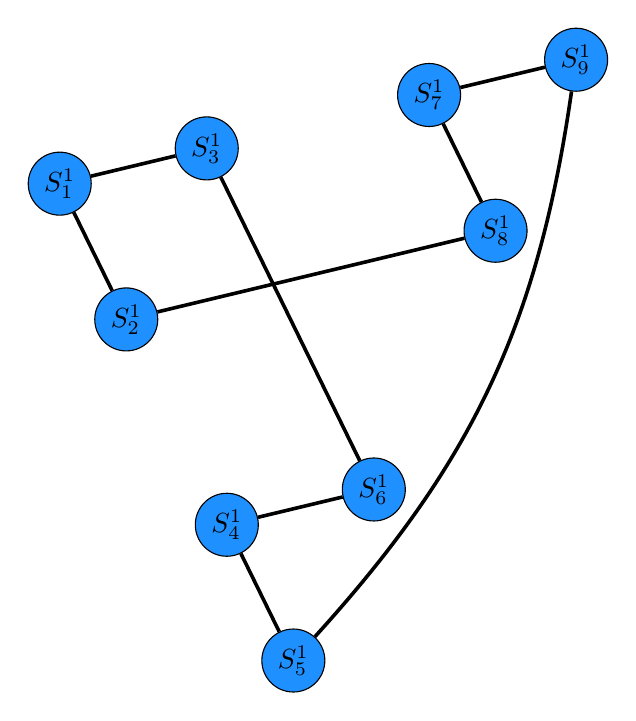
\begin{tikzpicture}[auto,vertex/.append style={minimum width=8mm}]
  \node[vertex,fill=DodgerBlue,text=black] (s1) at (0.000, -0.000) {$S_1^1$};
  \node[vertex,fill=DodgerBlue,text=black] (s2) at (0.845, -1.724) {$S_2^1$};
  \node[vertex,fill=DodgerBlue,text=black] (s3) at (1.867, 0.448) {$S_3^1$};
  \node[vertex,fill=DodgerBlue,text=black] (s4) at (2.122, -4.332) {$S_4^1$};
  \node[vertex,fill=DodgerBlue,text=black] (s5) at (2.967, -6.056) {$S_5^1$};
  \node[vertex,fill=DodgerBlue,text=black] (s6) at (3.989, -3.884) {$S_6^1$};
  \node[vertex,fill=DodgerBlue,text=black] (s7) at (4.691, 1.126) {$S_7^1$};
  \node[vertex,fill=DodgerBlue,text=black] (s8) at (5.535, -0.598) {$S_8^1$};
  \node[vertex,fill=DodgerBlue,text=black] (s9) at (6.558, 1.574) {$S_9^1$};

  \foreach \source/\dest in {1/2, 1/3, 2/8,3/6,4/5,4/6,7/8,7/9}
  \draw[edge] (s\source) -- (s\dest);
  \draw[edge] (s5) edge [bend left =-17]  (s9);
\end{tikzpicture}
\end{document}
